%
% Chapter 10
%

\chapter{SYSTEMATIC UNCERTAINTIES}
Systematic uncertainties, often referred to as ``systematics'' arise from the uncertainty assigned to specific components of the signal
and background predictions. These components are categorized as either theoretical uncertainties associated with MC event generators, scale factor uncertainties
related to data and MC yields, data-driven background uncertainties, and finally miscellaneous shape uncertainties.  

Systematic uncertainties are accounted for in the maximum likelihood fit in the form of nuisance parameters. Each nuisance represents a systematic uncertainty
and affects either the overall normalization of the discriminant, known as a rate systematic, or the shape of the discriminant,
known as a shape systematic\footnote{Some shape systematics also vary the overall normalization}. The rate uncertainty scales all bins of the discriminant
by a constant factor, while the shape uncertainty varies individual bins separately, thus changing the shape of the discriminant.
The rate uncertainties use a log-normal prior, while the shape uncertainties use a gaussian prior. 

The correlations, or lack thereof, of each of the 274 nuisances in this analysis are accounted for in the likelihood fit. 
Rate uncertainties arising from the same source, are treated as fully correlated across event categories. Shape uncertainties are fully correlated between
bins of the discrmininant in each category. The bin-by-bin shape uncertainties, which account for limitied statistics, are treated as uncorrelated. 


\section{Theoretical Uncertainties}
The theoretical uncertainties in this analysis arise from the NLO calculation of the cross section for the signal and background processes.
All theoretical uncertainties propagated as into the fit as rate uncertainties. For \tth signal,
these uncertainties amount to +5.8$\%$ -9.2$\%$ from unknown higher order terms in the perturbative expansion and an additional 3.6$\%$ uncertainty for the
PDFs and the scale ($\alpha_{s}$). For the leading MC background of \ttw and \ttz, the cross section uncertainties are 12$\%$ and 10$\%$ respectively, with
scale uncertainties of 2$\%$ and 3$\%$ respectively~\cite{xsec_uncert}. A conservative 50$\%$ uncertainty is assigned to all other background MC processes. 

\section{Scale Factor Uncertainties}
Scale factor systematics represent the uncertainty associated with the agreement between data and MC in a given observable. In this analysis,
scale factor uncertainties enter the fit in the form of both rate and shape systematics. Scale factor uncertainties are assesed for trigger efficiency,
lepton selection efficieny, b-tagging efficiency. The trigger efficiency scale factors show nearly perfect agreement, and have uncertainties of approximately
2$\%$ - which is propagated as a rate uncertainty. The uncertainties on the scale factors for b-tagging are assessed for both heavy flavor and light flavor separately,
and the b-tag weights are adjusted by $\pm$1 $\sigma$ depending on the specific b-tagging uncertainty and propagated to the fit as shape uncertainties.
These uncertainties amount to around 3$\%$ for b-tagging, and 10$\%$ for mistag rates.

\section{Data-driven Background Uncertainties}
The uncertainties associated with the data-driven background control regions are the dominant systematics in this analysis. 
Several checks on the data/MC agreement are performed in the control regions to confirm that the data-driven methods are accurate for the reducible MC-estimated
backgrounds. These checks are performed for the backgrounds arising from fake leptons and charge flips separately.

For the background due to fake leptons, an alternative fake rare is extracted from non-prompt leptons in QCD MC, and applied to 2lss semi-leptonic \ttbar MC events in the application region.
Additionally, a second MC fake rate from non-prompt leptons in $\ttbar$ MC,  is applied to the same 2lss sample.
The test described above is performed in each of the signal regions described above. 
The difference in normalization between the two fake rate predictions, as well as the difference in discriminant against the $\ttbar$ and ttV backgrounds,
are propagated as a shape uncertainty to the fit. Examples of these shape variations are in Figures~\ref{fig:closure}.
The rate uncertainties from the data/MC agreement of the electron (muon) fake rates range from 10\% to 30\% (from 20\% to 40\%) depending on the analysis category,
and are larger in the b-tight categories. Separate nuisance parameters account for the normalization in the b-loose and b-tight categories, and for different lepton flavors.
Shape uncertainties are propaged at fixed normalization, and accounted for in the fit with linear distortions acting simultaneously on the two axes of the 2D BDT plane.
The slope of the distortion typically ranges from 0.1 to 0.4, with separate nuisances for b-loose and b-tight categories, and for different lepton flavors.

\begin{figure}[htb]
        \centering 
        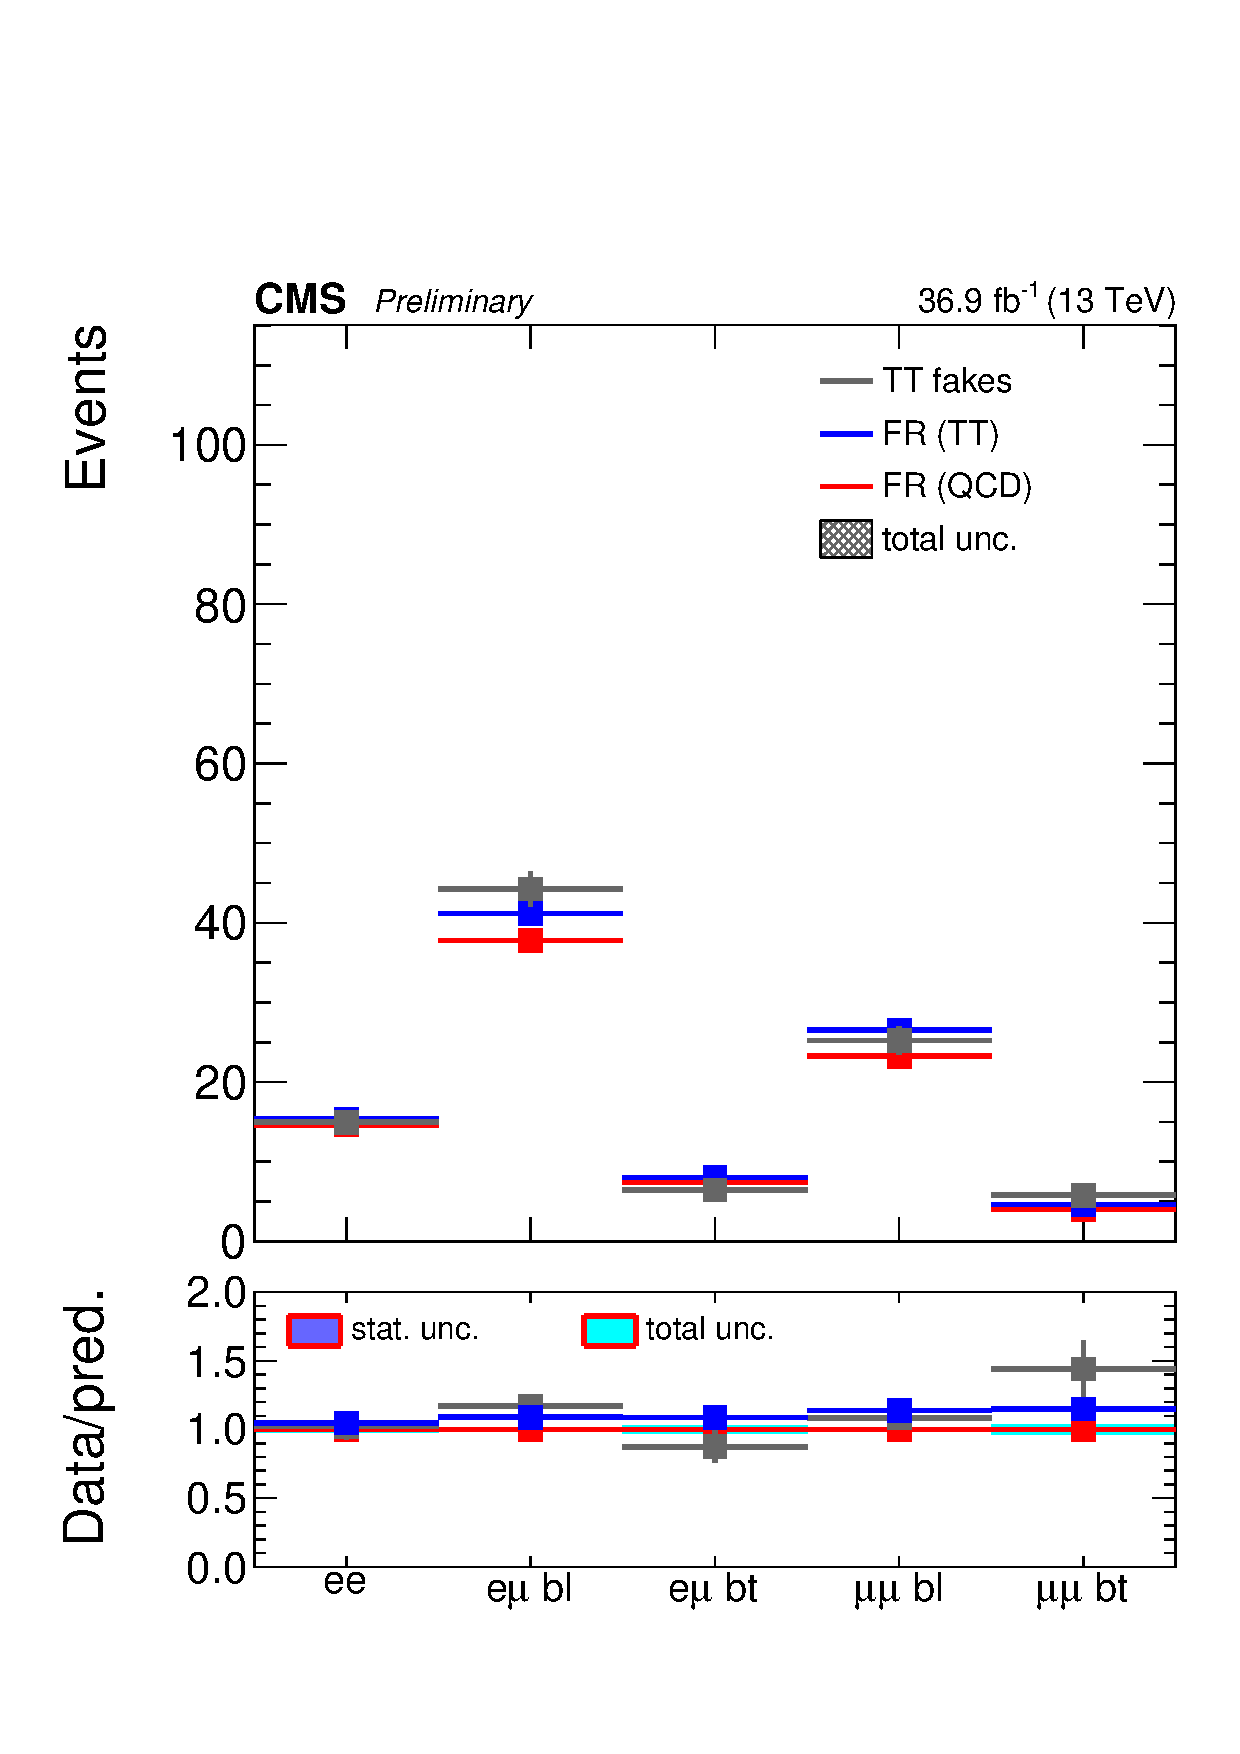
\includegraphics[width=0.32\textwidth]{ch10_figs/2lep_catIndex_nosign.pdf}
        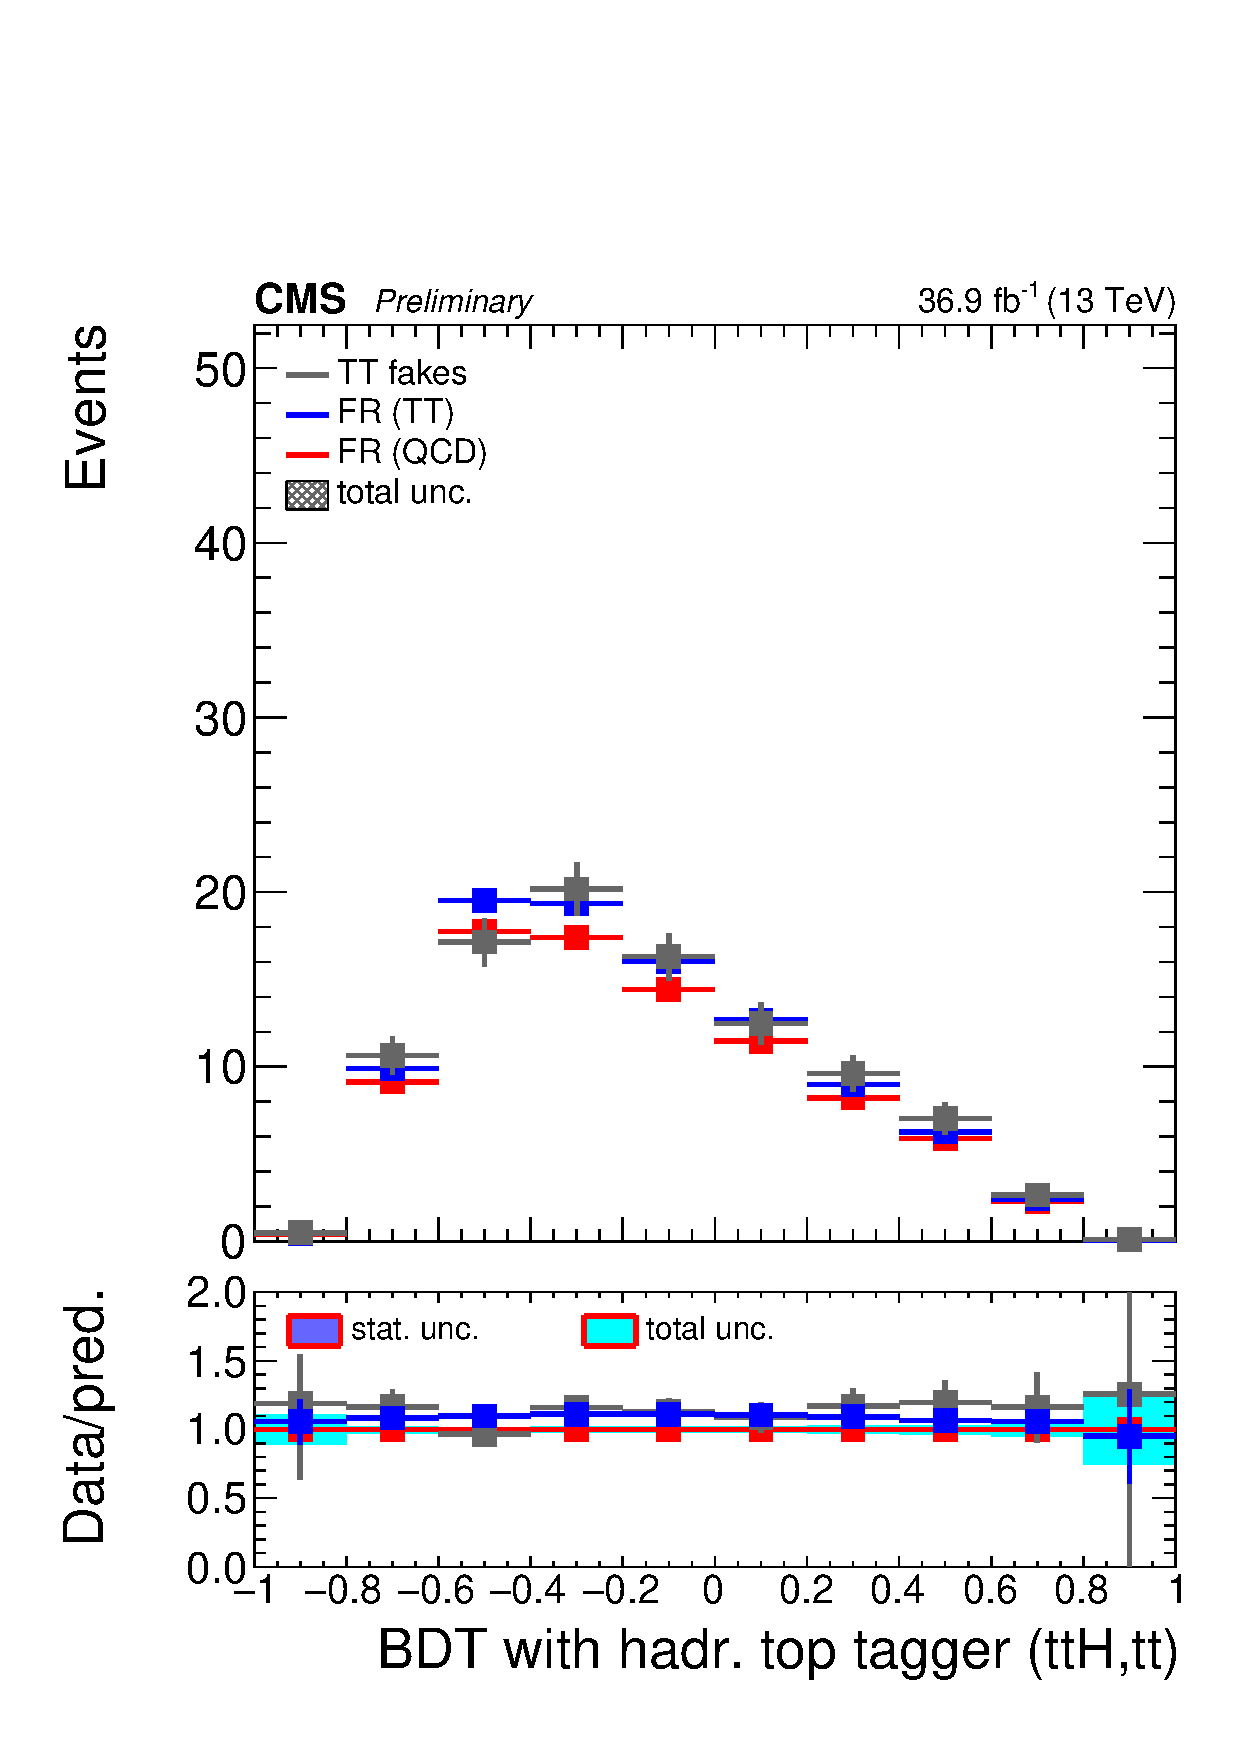
\includegraphics[width=0.32\textwidth]{ch10_figs/kinMVA_2lss_ttbar_withBDTv8.pdf}
        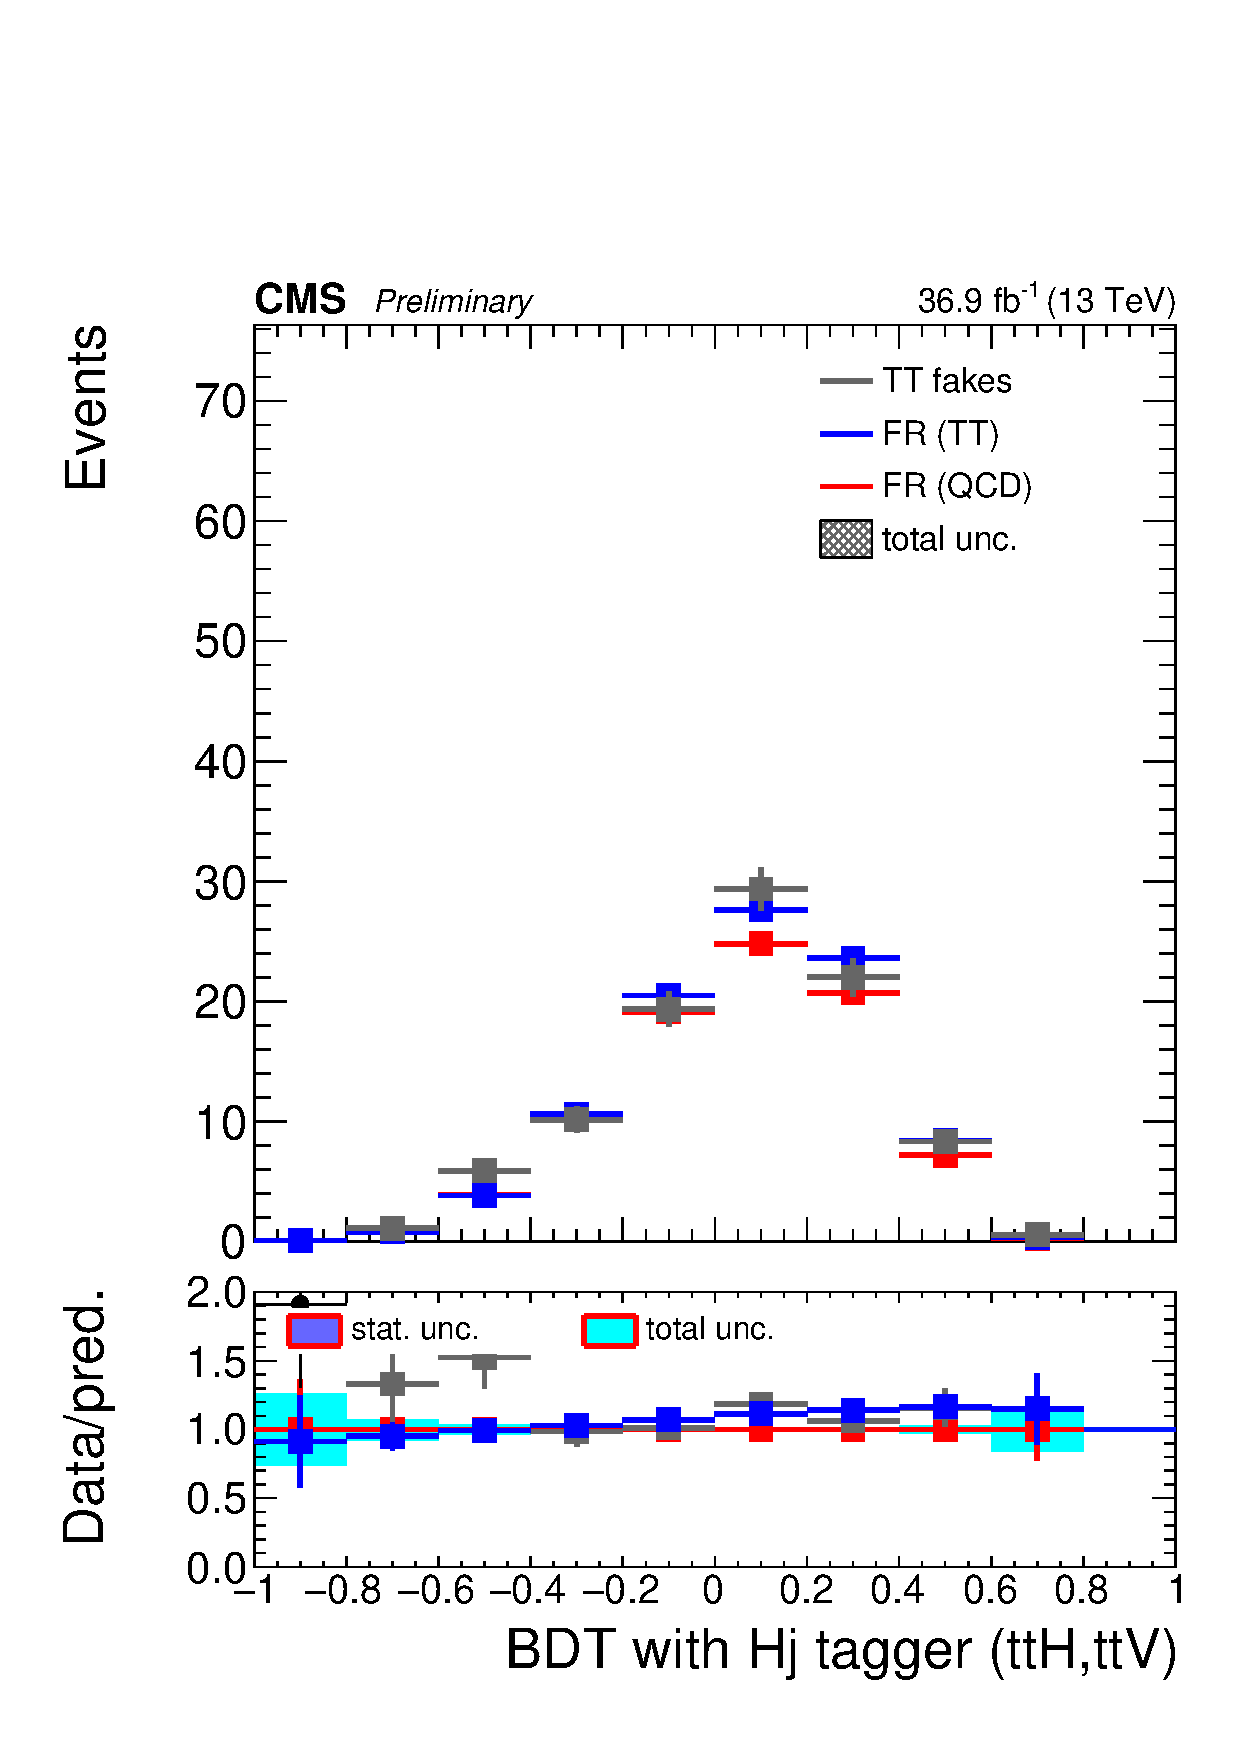
\includegraphics[width=0.32\textwidth]{ch10_figs/kinMVA_2lss_ttV_withHj.pdf}
        \caption[MC validation plots of FR method]{Distributions of semi-leptonic $\ttbar$ MC in the signal region, compared with background predictions obtained
          in MC using fake rates extracted in QCD and $\ttbar$ MC events.}
        \label{fig:closure}
\end{figure}

\noindent The uncertainty on the fake rate measurement is propagated to the fit with several nuisances that vary both
the background normalization with a rate systematic, and the background shape by introducing trends
in the fake rate bins as a function of the lepton $\pt$ and $|\eta|$  at fixed normalization.
This is done separately for electrons and muons. These variations are below in Figure~\ref{fig:FRvars_shape}.

\begin{figure}[htb]
        \centering 
        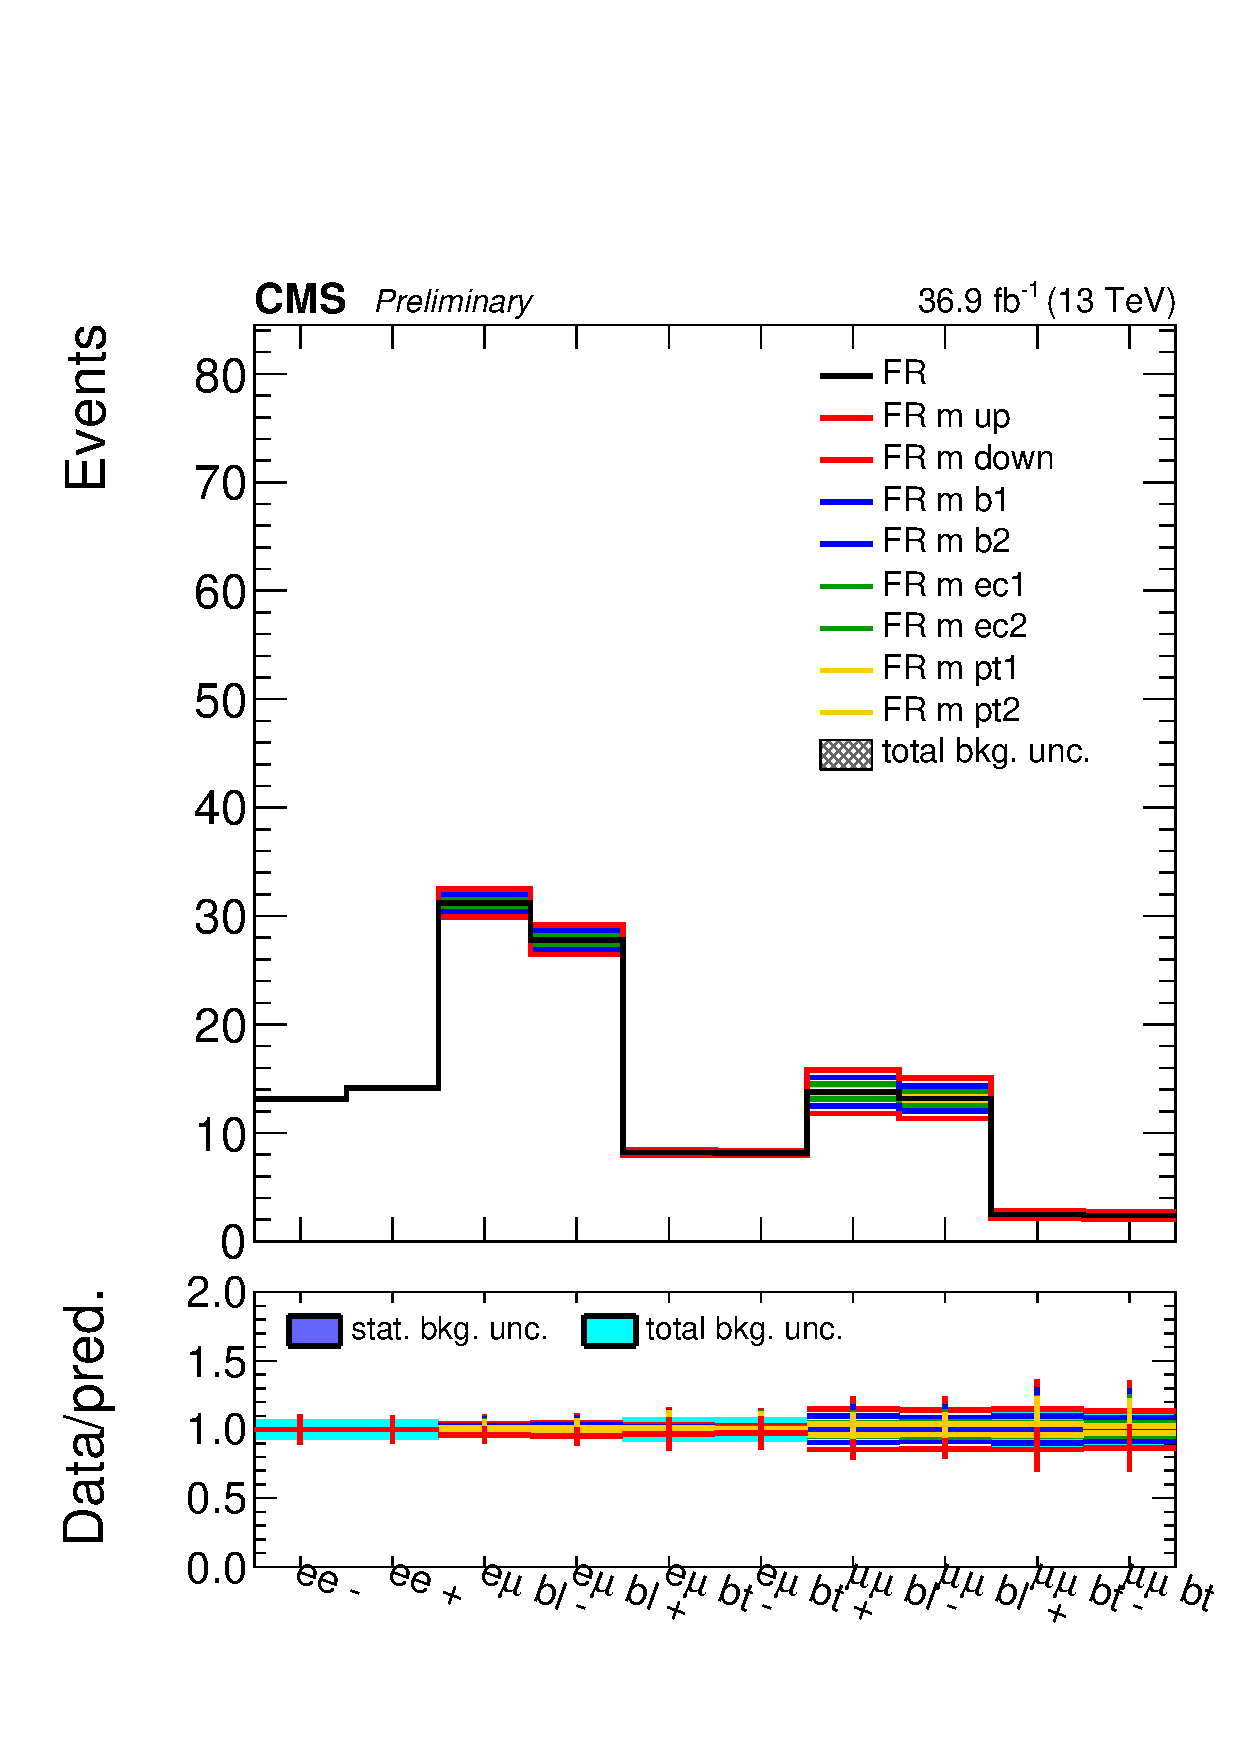
\includegraphics[width=0.32\textwidth]{ch10_figs/2lep_mu_catIndex.pdf}
        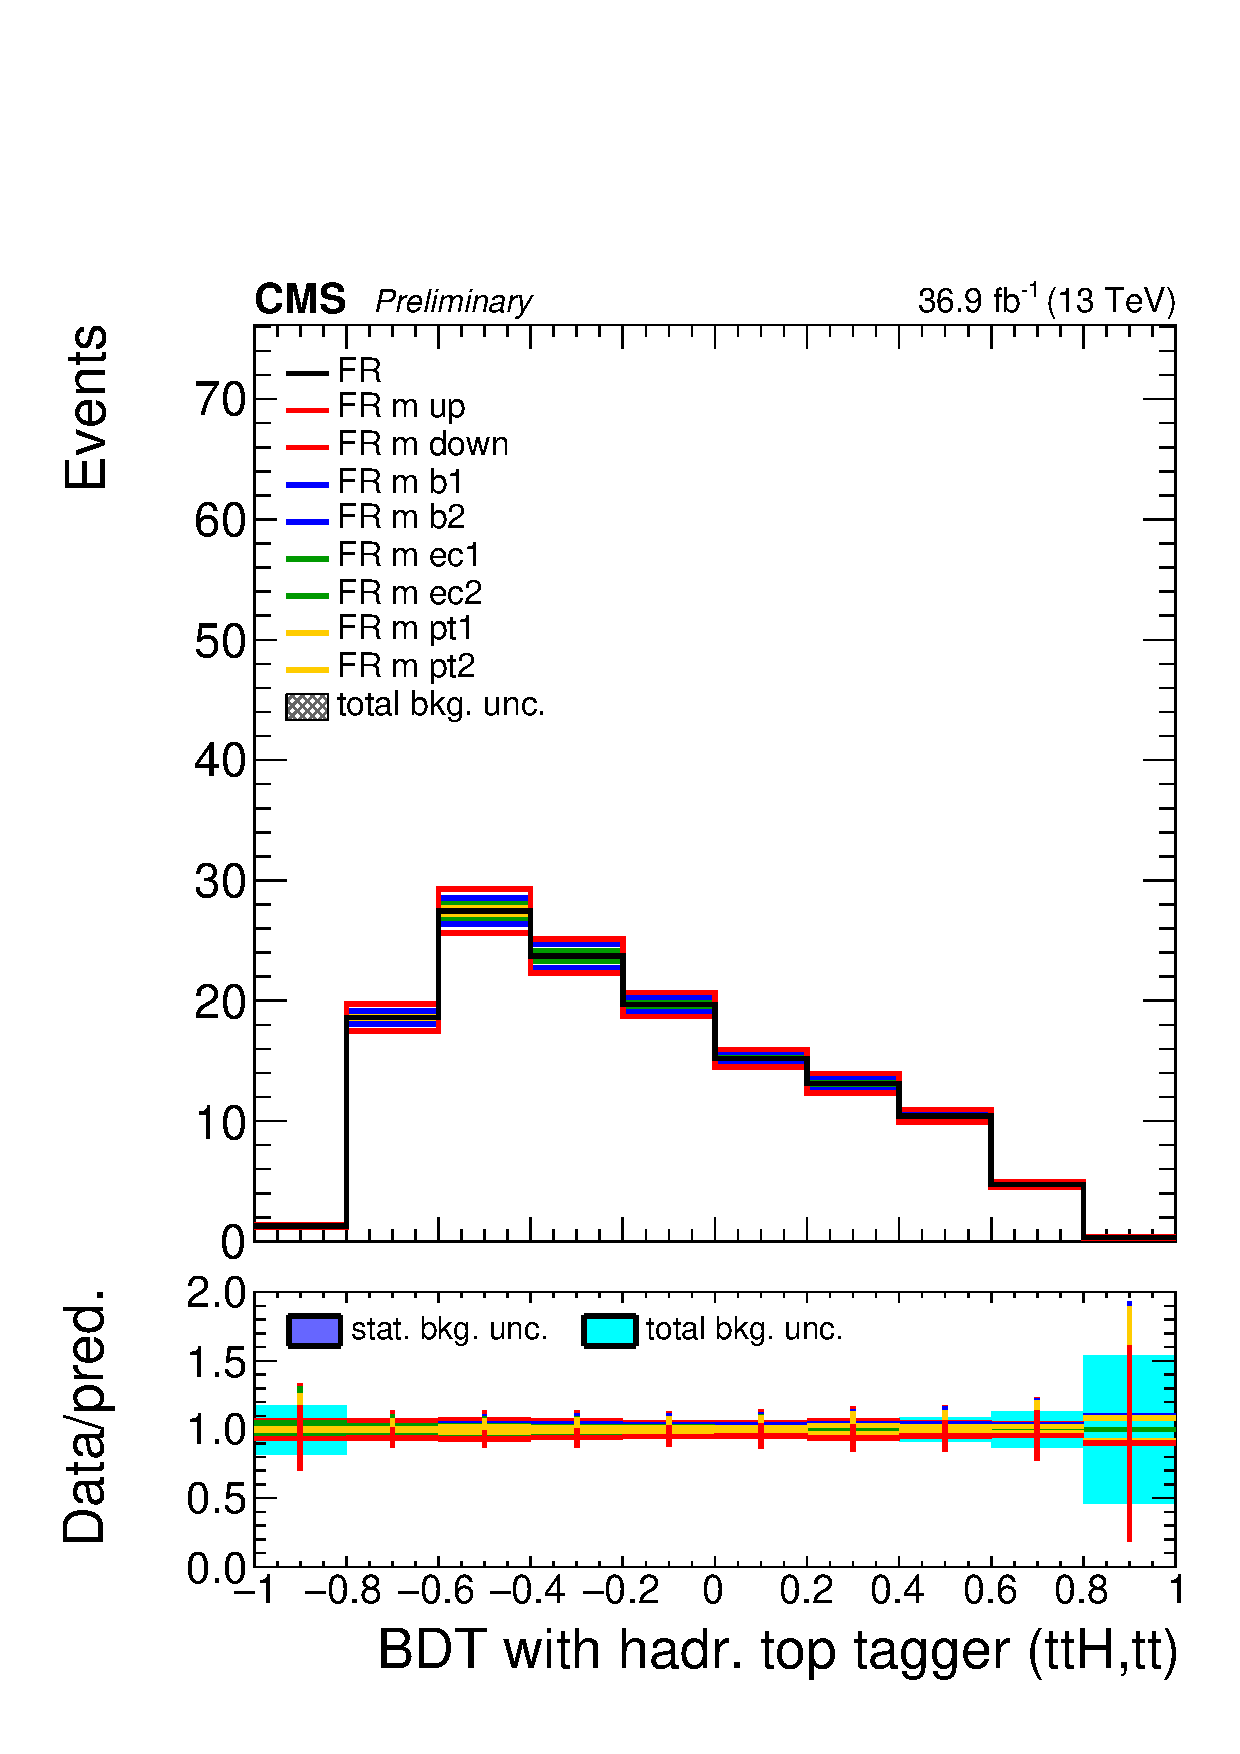
\includegraphics[width=0.32\textwidth]{ch10_figs/kinMVA_2lss_mu_ttbar_withBDTv8.pdf}
        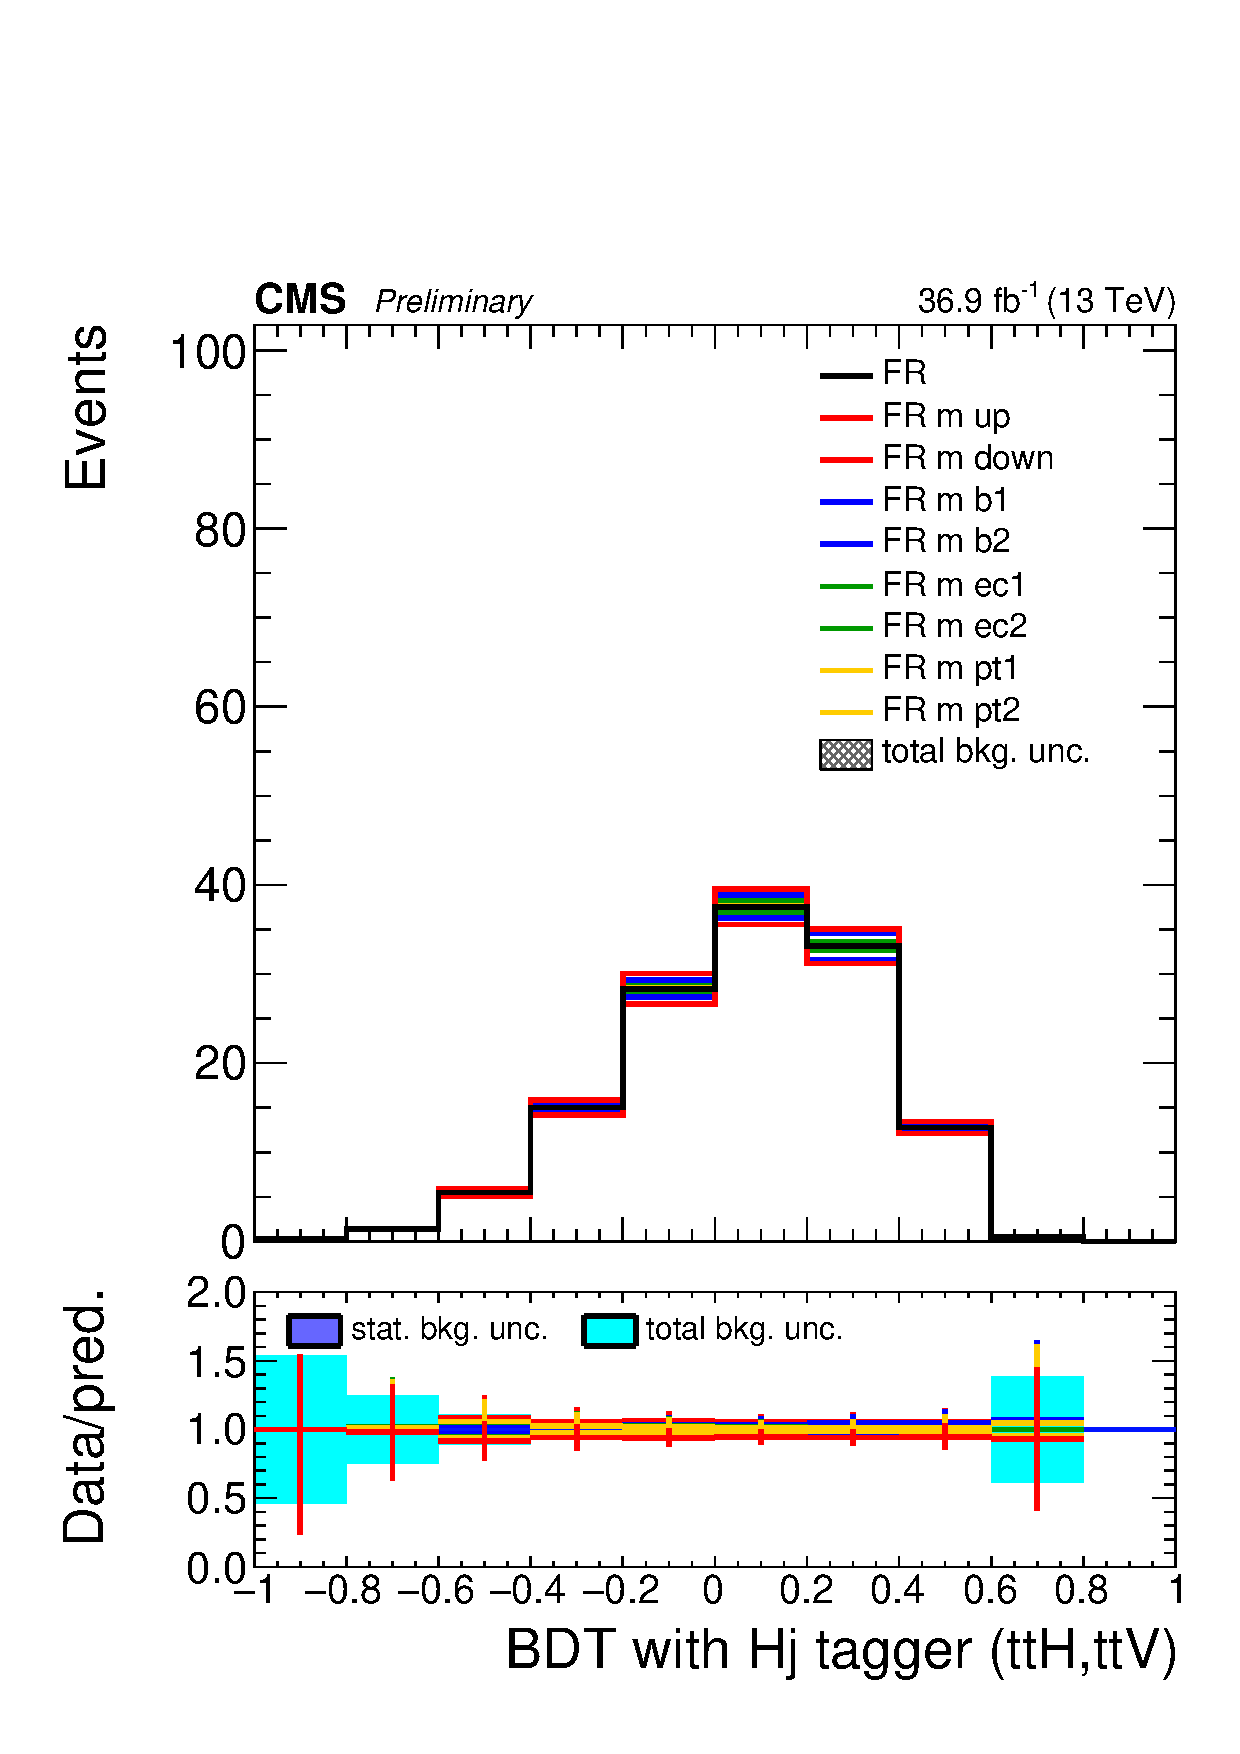
\includegraphics[width=0.32\textwidth]{ch10_figs/kinMVA_2lss_mu_ttV_withHj.pdf}\\
        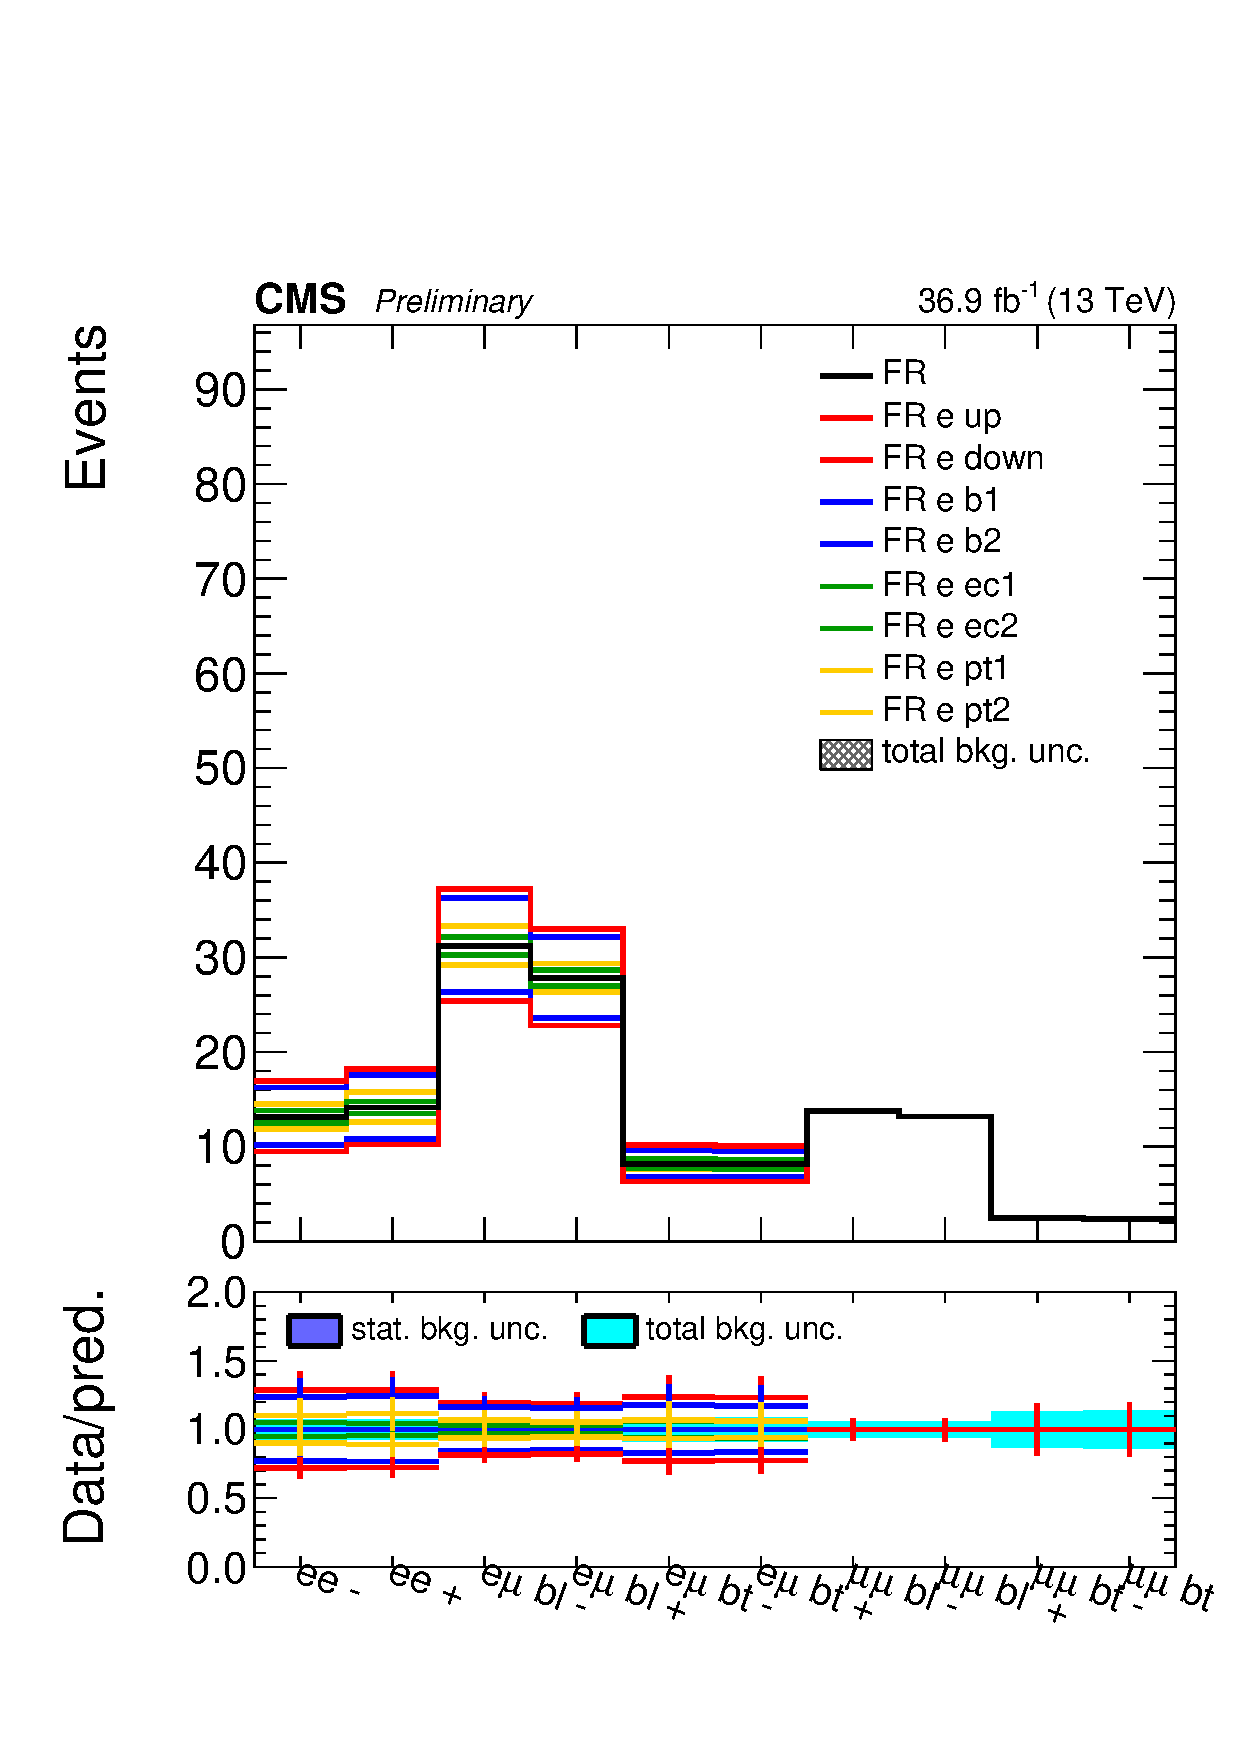
\includegraphics[width=0.32\textwidth]{ch10_figs/2lep_e_catIndex.pdf}
        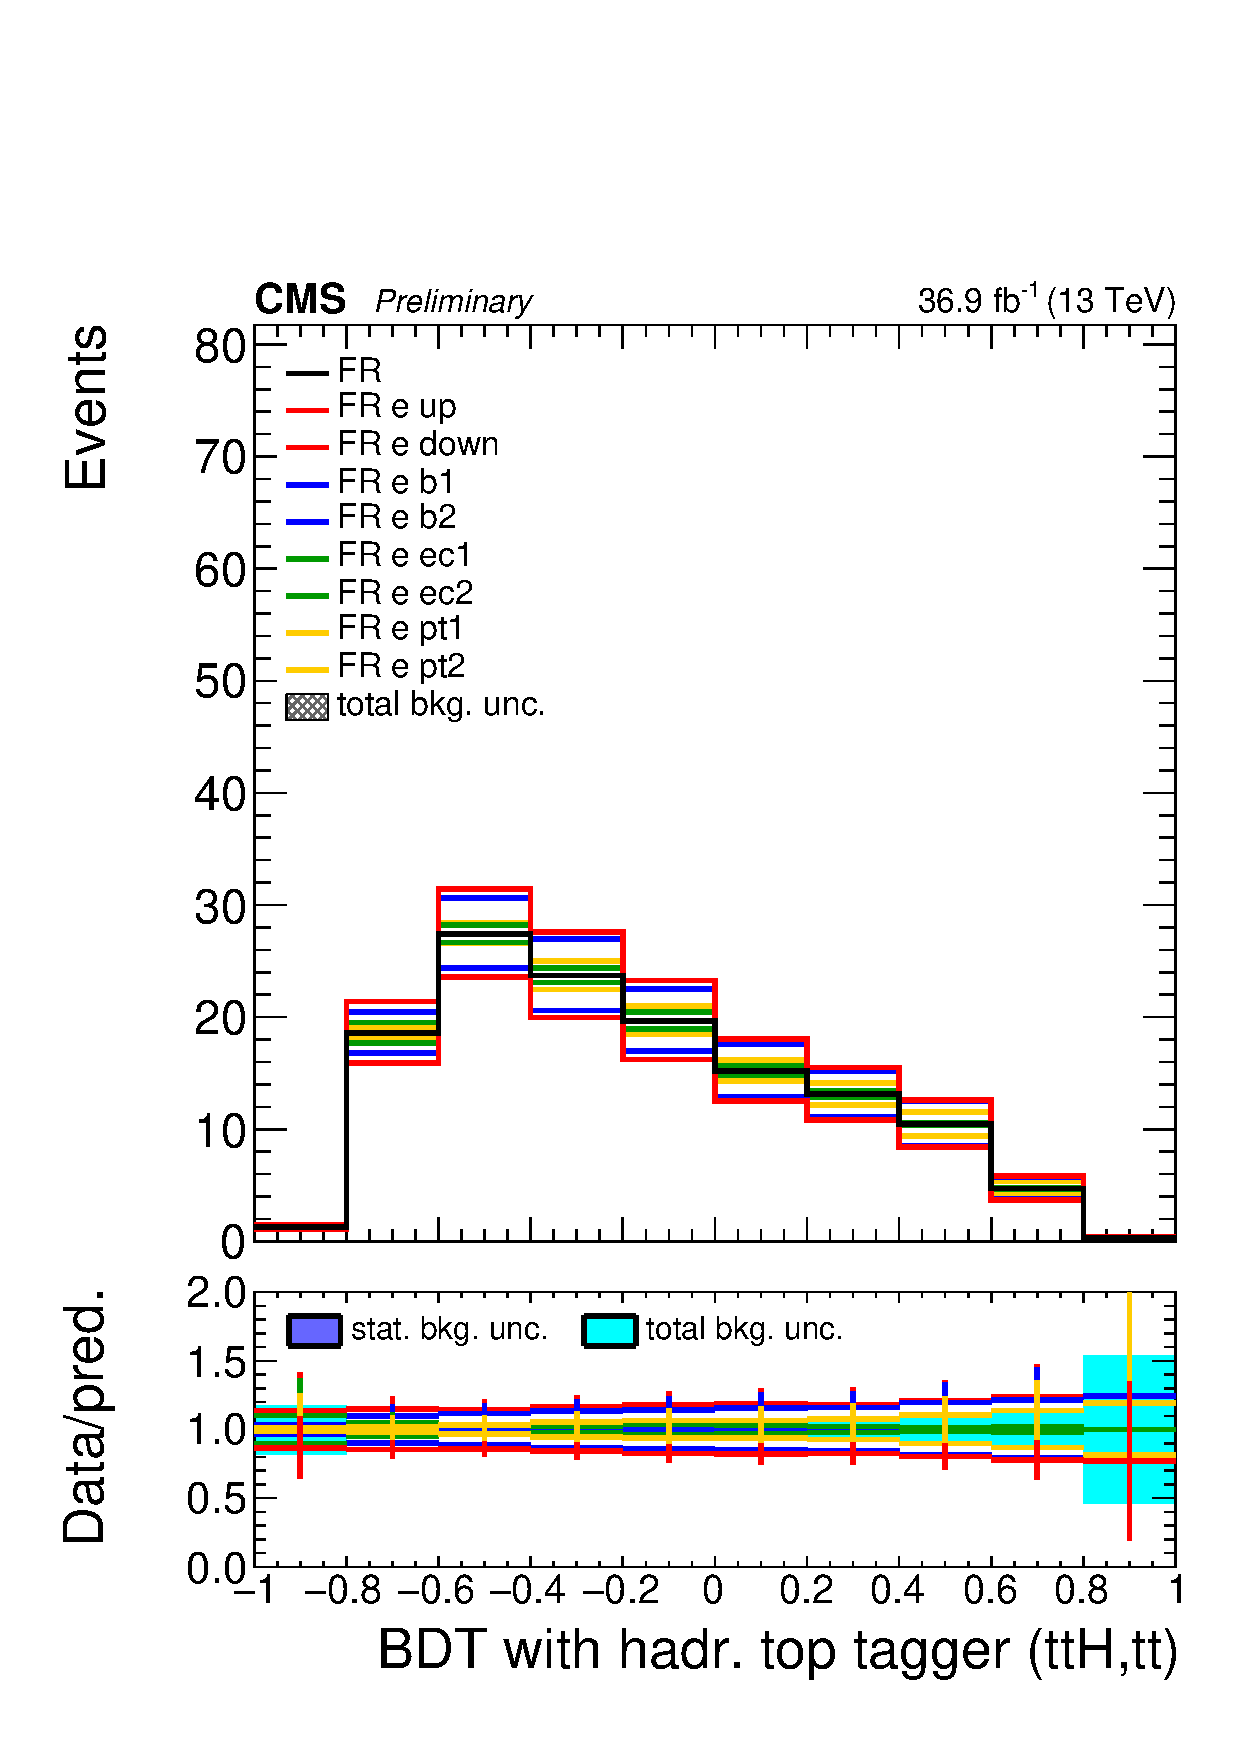
\includegraphics[width=0.32\textwidth]{ch10_figs/kinMVA_2lss_e_ttbar_withBDTv8.pdf}
        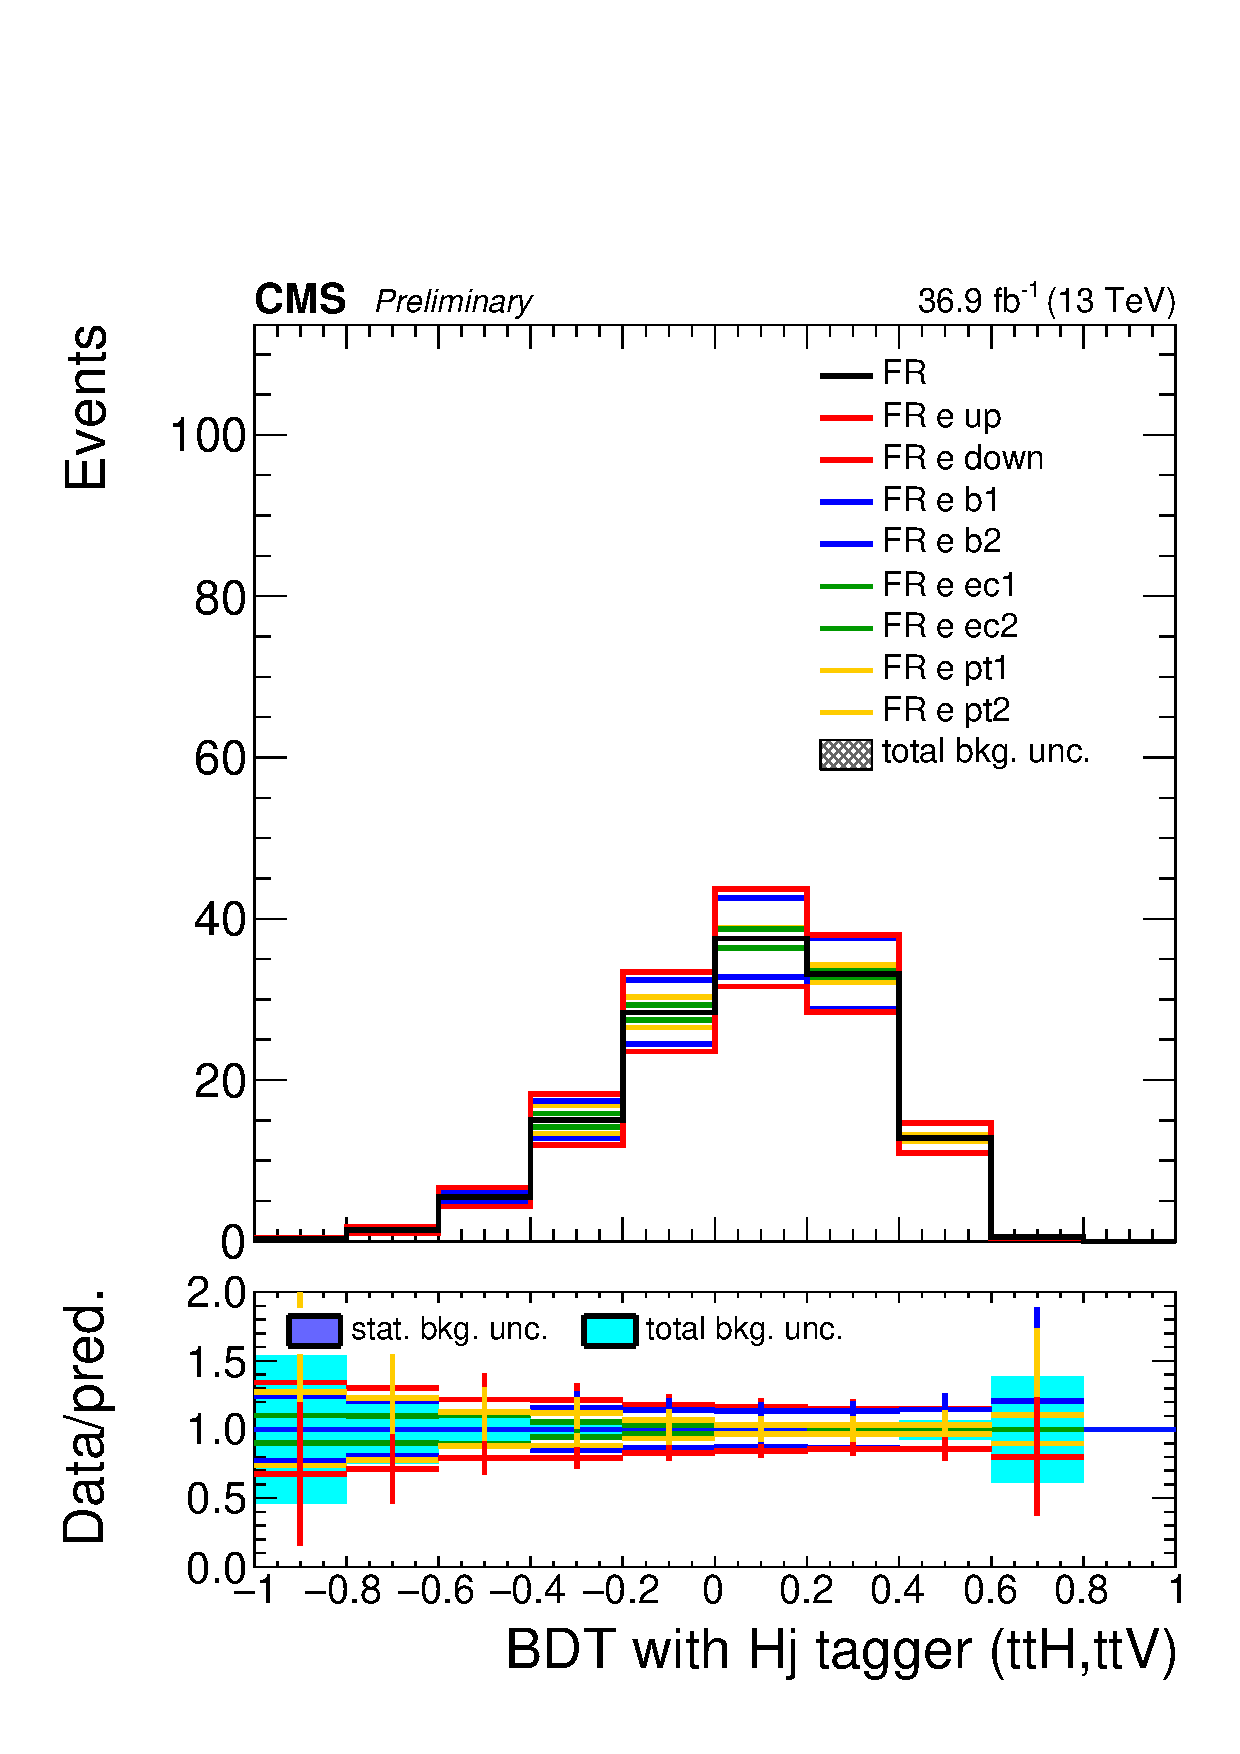
\includegraphics[width=0.32\textwidth]{ch10_figs/kinMVA_2lss_e_ttV_withHj.pdf}
        \caption{Background shape variations from shifts and distortions of the measured data fake rate bins within uncertainties. 
          Rate normalization shifts are in red. barrel, endcap region shifts are in blue, green respectively. Variations as a function
          of lepton \pt are in yellow. The top,bottom row is for variations to the muon,electron fake rates respectively.}
        \label{fig:FRvars_shape}
\end{figure}

For the background due to charge mis-assignments, the estimation method is validated in two separate control regions.
The first is the control region used for measuring the chare flip rates, and the second is enriched in \ttbar events, with the same b-jet
requirement as the signal region, and 2 or 3 preselected jets. Based on the statistical uncertainty of measured probabilities
and the closure with data in the validation control regions, a 30$\%$ uncertainty is assigned to this background. 



\section{Misc. Shape Uncertainties}
Miscellaneous shape uncertainties not falling into the above categories include some of the most important systematics in the analysis.
These systematics include the uncertainty on the jet energy corrections, which  shift the weight of each jet up and down
by $\pm$1$\sigma$ and re-calculating the signal region yields. To account for statistical fluctuations in individual bins, shape systematics
are assigned that vary each individual bin in each category for each process. 




%% \begin{figure}[hbtp]
%%  \begin{center}
%%    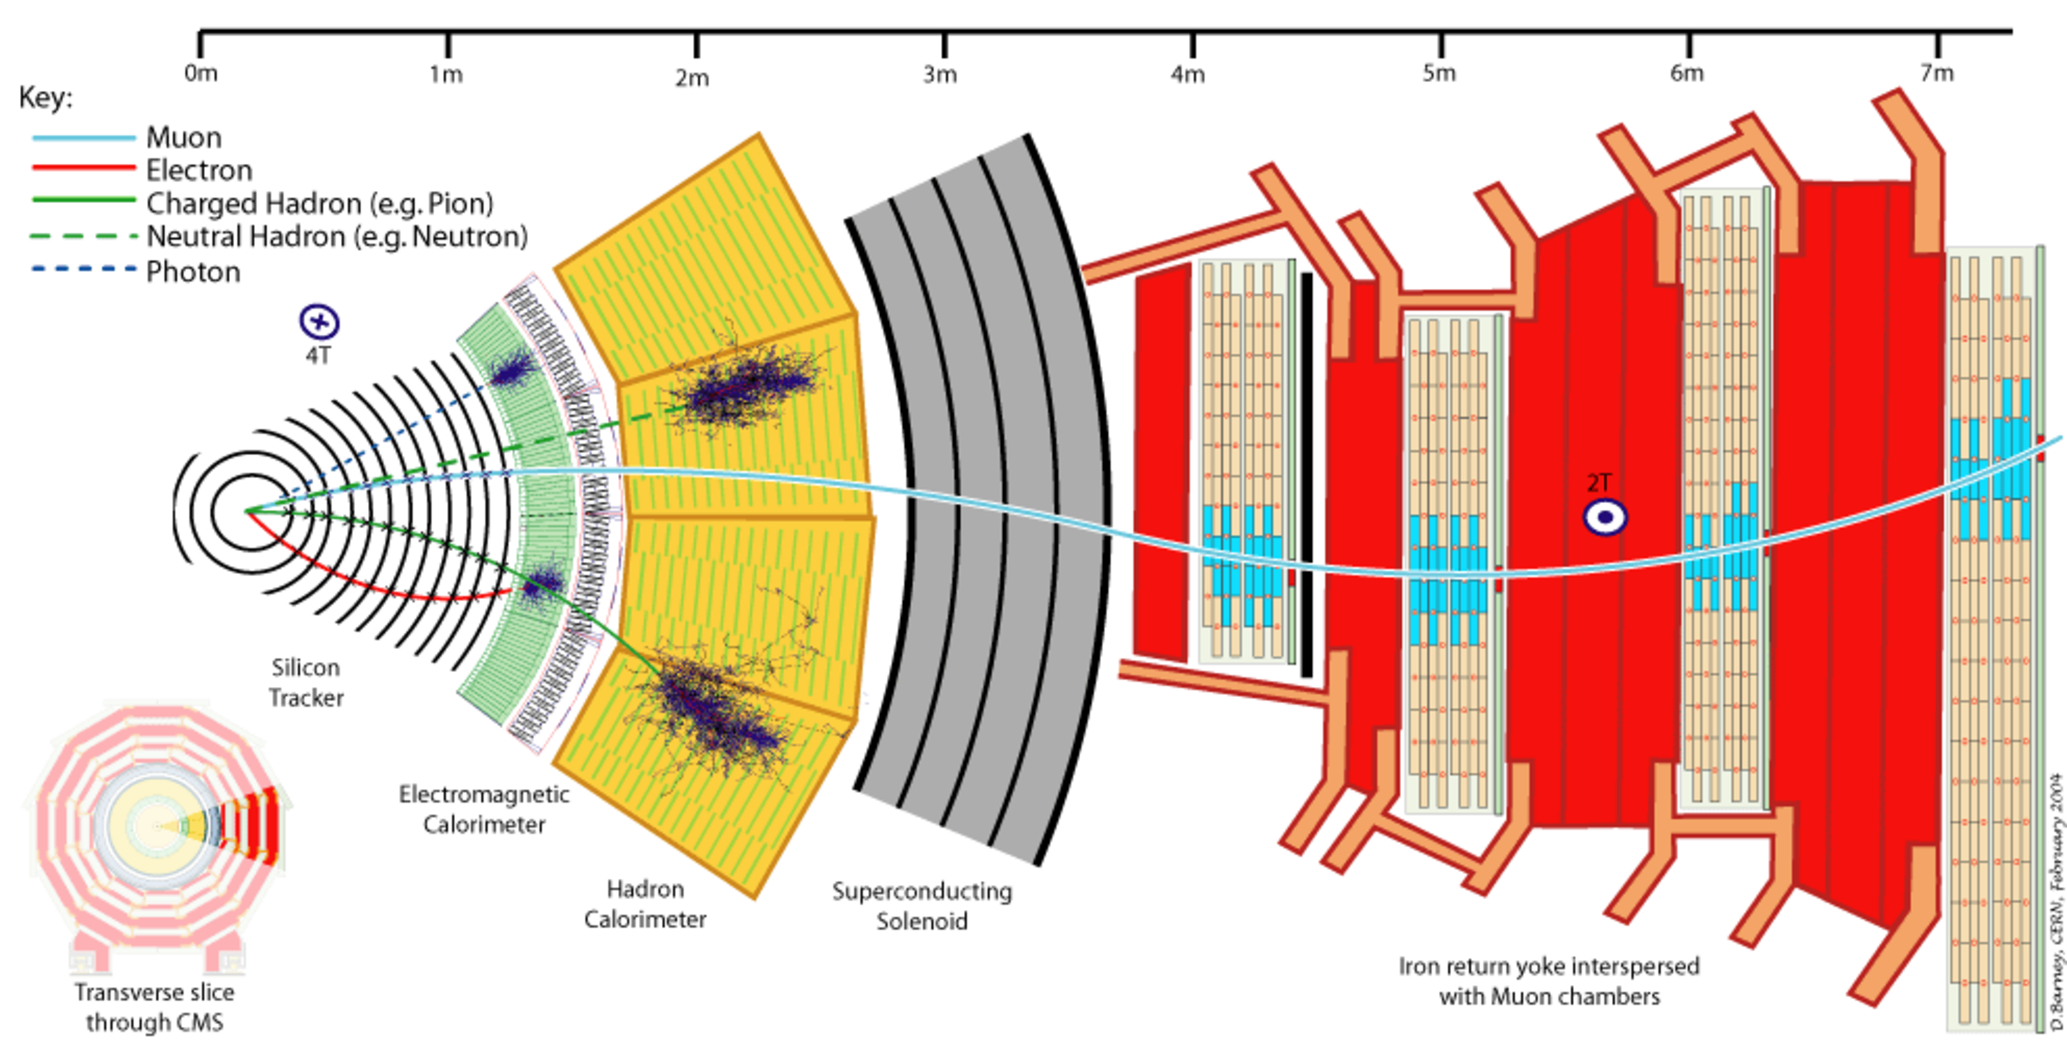
\includegraphics[width=0.8\textwidth]{ch4_figs/cms_particleflow.pdf}
%%    \caption{An overview of how CMS detects different types of particles. The slice of CMS in in the x-y plane.~\cite{NEED CITATION}.}
%%    \label{fig:cms_pflow}
%%  \end{center}
%% \end{figure}
